\documentclass[11pt,a4paper,titlepage]{article}
\usepackage[utf8]{inputenc}
\usepackage[english]{babel}
\usepackage{lipsum}
\usepackage[a4paper, top=2.5cm, bottom=2.5cm, left=2.2cm, right=2.2cm]{geometry}


\usepackage{amsmath, amssymb, amsfonts, amsthm, fouriernc, mathtools}
% mathtools for: Aboxed (put box on last equation in align envirenment)
\usepackage{microtype} %improves the spacing between words and letters

\usepackage{graphicx}
\graphicspath{ {./pics/} {./eps/}}
\usepackage{epsfig}
\usepackage{epstopdf}


%%%%%%%%%%%%%%%%%%%%%%%%%%%%%%%%%%%%%%%%%%%%%%%%%%
%% COLOR DEFINITIONS
%%%%%%%%%%%%%%%%%%%%%%%%%%%%%%%%%%%%%%%%%%%%%%%%%%
\usepackage[svgnames]{xcolor} % Enabling mixing colors and color's call by 'svgnames'
%%%%%%%%%%%%%%%%%%%%%%%%%%%%%%%%%%%%%%%%%%%%%%%%%%
\definecolor{MyColor1}{rgb}{0.2,0.4,0.6} %mix personal color
\newcommand{\textb}{\color{Black} \usefont{OT1}{lmss}{m}{n}}
\newcommand{\blue}{\color{MyColor1} \usefont{OT1}{lmss}{m}{n}}
\newcommand{\blueb}{\color{MyColor1} \usefont{OT1}{lmss}{b}{n}}
\newcommand{\red}{\color{LightCoral} \usefont{OT1}{lmss}{m}{n}}
\newcommand{\green}{\color{Turquoise} \usefont{OT1}{lmss}{m}{n}}
%%%%%%%%%%%%%%%%%%%%%%%%%%%%%%%%%%%%%%%%%%%%%%%%%%




%%%%%%%%%%%%%%%%%%%%%%%%%%%%%%%%%%%%%%%%%%%%%%%%%%
%% FONTS AND COLORS
%%%%%%%%%%%%%%%%%%%%%%%%%%%%%%%%%%%%%%%%%%%%%%%%%%
%    SECTIONS
%%%%%%%%%%%%%%%%%%%%%%%%%%%%%%%%%%%%%%%%%%%%%%%%%%
\usepackage{titlesec}
\usepackage{sectsty}
%%%%%%%%%%%%%%%%%%%%%%%%
%set section/subsections HEADINGS font and color
\sectionfont{\color{MyColor1}}  % sets colour of sections
\subsectionfont{\color{MyColor1}}  % sets colour of sections

%set section enumerator to arabic number (see footnotes markings alternatives)
\renewcommand\thesection{\arabic{section}.} %define sections numbering
\renewcommand\thesubsection{\thesection\arabic{subsection}} %subsec.num.

%define new section style
\newcommand{\mysection}{
\titleformat{\section} [runin] {\usefont{OT1}{lmss}{b}{n}\color{MyColor1}} 
{\thesection} {3pt} {} } 

%%%%%%%%%%%%%%%%%%%%%%%%%%%%%%%%%%%%%%%%%%%%%%%%%%
%		CAPTIONS
%%%%%%%%%%%%%%%%%%%%%%%%%%%%%%%%%%%%%%%%%%%%%%%%%%
\usepackage{caption}
\usepackage{subcaption}
%%%%%%%%%%%%%%%%%%%%%%%%
\captionsetup[figure]{labelfont={color=Turquoise}}

%%%%%%%%%%%%%%%%%%%%%%%%%%%%%%%%%%%%%%%%%%%%%%%%%%
%		!!!EQUATION (ARRAY) --> USING ALIGN INSTEAD
%%%%%%%%%%%%%%%%%%%%%%%%%%%%%%%%%%%%%%%%%%%%%%%%%%
%using amsmath package to redefine eq. numeration (1.1, 1.2, ...) 
%%%%%%%%%%%%%%%%%%%%%%%%
\renewcommand{\theequation}{\thesection\arabic{equation}}

%set box background to grey in align environment 
\usepackage{etoolbox}% http://ctan.org/pkg/etoolbox
\makeatletter
\patchcmd{\@Aboxed}{\boxed{#1#2}}{\colorbox{black!15}{$#1#2$}}{}{}%
\patchcmd{\@boxed}{\boxed{#1#2}}{\colorbox{black!15}{$#1#2$}}{}{}%
\makeatother
%%%%%%%%%%%%%%%%%%%%%%%%%%%%%%%%%%%%%%%%%%%%%%%%%%




%%%%%%%%%%%%%%%%%%%%%%%%%%%%%%%%%%%%%%%%%%%%%%%%%%
%% DESIGN CIRCUITS
%%%%%%%%%%%%%%%%%%%%%%%%%%%%%%%%%%%%%%%%%%%%%%%%%%
\usepackage[siunitx, american, smartlabels, cute inductors, europeanvoltages]{circuitikz}


\makeatletter
\let\reftagform@=\tagform@
\def\tagform@#1{\maketag@@@{(\ignorespaces\textcolor{red}{#1}\unskip\@@italiccorr)}}
\renewcommand{\eqref}[1]{\textup{\reftagform@{\ref{#1}}}}
\makeatother
\usepackage{hyperref}
\hypersetup{colorlinks=true}

\title{ CS $215$ 

\blueb Homework $1$}
\author{
  Omkar Shirpure\\
  \texttt{22B0910}
  \and
  Krish Rakholiya\\
  \texttt{22B0927}
}
\date{}
%%%%%%%%%%%%%%%%%%%%%%%%%%%%%%%%%%%%%%%%%%%%%%%%%%



\begin{document}
\maketitle

\section{Question 1 : }{
\subsection{}{
The probability of the every person picking their own notebook is (for the first person to get his own notebook is $\frac{1}{n}$, for the second person $\frac{1}{n-1}$ and so on... ) 

So their overall probability is
$$P = \frac{1}{n}*\frac{1}{n-1} ... \frac{1}{2}*\frac{1}{1}$$
Hence,
$$P = \frac{1}{n!}$$
}

\subsection{}{
The probability of getting the correct notebooks for the first m(<n) people could be calculated by same method. W.K.T. (for the first person to get his own notebook is $\frac{1}{n}$, for the second person $\frac{1}{n-1}$ up to $m$th person $\frac{1}{n-m+1}$)

\vspace{0.2cm}
The overall probability will be
$$P = (\frac{1}{n})(\frac{1}{n-1})(\frac{1}{n-2})...(\frac{1}{n-m+1})$$
$$P = \frac{1}{(n-m)!}$$
$$P = \binom{n}{m}^{-1}$$
}

\subsection{}{
This is conceptually same as the previous one, where just the set of $m$ changes from first to last.
Hence,
$$P = \frac{1}{(n-m)!}$$
$$P = \binom{n}{m}^{-1}$$
}

\subsection{}{
The probability of getting clean books for first $m$ persons is 
$$P = (1-p)^m$$
since the probability of book being clean is independent of any other factors.
}

\subsection{}{
Since it is given that first $m$ persons pick up clean books (with probability (1-p)) and rest of the $(n-m)$ people pick up unclean books (with probability p).
The total probability is 
$$P = \binom{n}{m}(1-p)^m(p)^{n-m}$$
}
\newpage
\section{Question 2 : }{
We are given n distinct values $x_i$ with their mean $\mu$ and standard deviation $\sigma$ and to prove 
$$|x_i-\mu| \leq \sigma \sqrt{n-1}$$
Since we defined the variance as 
$$\sigma^2 = \frac{\Sigma(x_i - \mu)^2}{n-1}$$
From the equation to prove, squaring on both sides and expanding, it gives,
$$(x_i - \mu)^2 \leq \sigma^2(n-1) $$
$$x_i^2 -2x_i\mu + \mu^2 \leq \sigma^2(n-1)$$
Taking expectation of both sides,
$$E(x_i^2) - 2\mu E(x_i) + \mu^2 \leq $$
$$E(x_i^2) - \mu^2 \leq \sigma^2(n-1)$$
Since, Var $ = E(x_i^2) - \mu^2$, substituting we get,
$${var} \leq \sigma^2(n-1)$$
$${var} \leq {var}(n-1)$$

And since, variance is always non-negative, this inequality holds true. And hence the inequality $|x_i-\mu| \leq \sigma \sqrt{n-1}$ holds true for all individual $x_i$. \\

Coming to comparison with Chebyshev's Inequality as $n$ increases, the above becomes a more stronger statement compared to Chebyshev's Inequality. Chebyshev's Inequality in general being just the probabilistic bound for all distributions, but the above inequality gives a direct relation between all the individual data points, and other details such as mean, standard deviation, etc.And as $n$ increases, the proven inequality becomes more accurate and informative for this specific data set as compared to Chebyshev's inequality.
}
\newpage
\section{Question 6 : }{
\textit{The code and plots for this question has been included in the folder.} \\
\begin{itemize}
    \item at $f = 30\%$
    \begin{itemize}
        \item The RMS error of moving median filtering is $15.186$.
        \item The RMS error of moving mean filtering is $58.9177$.
        \item The RMS error of moving quartile filtering is $0.015119$.
    \end{itemize}
    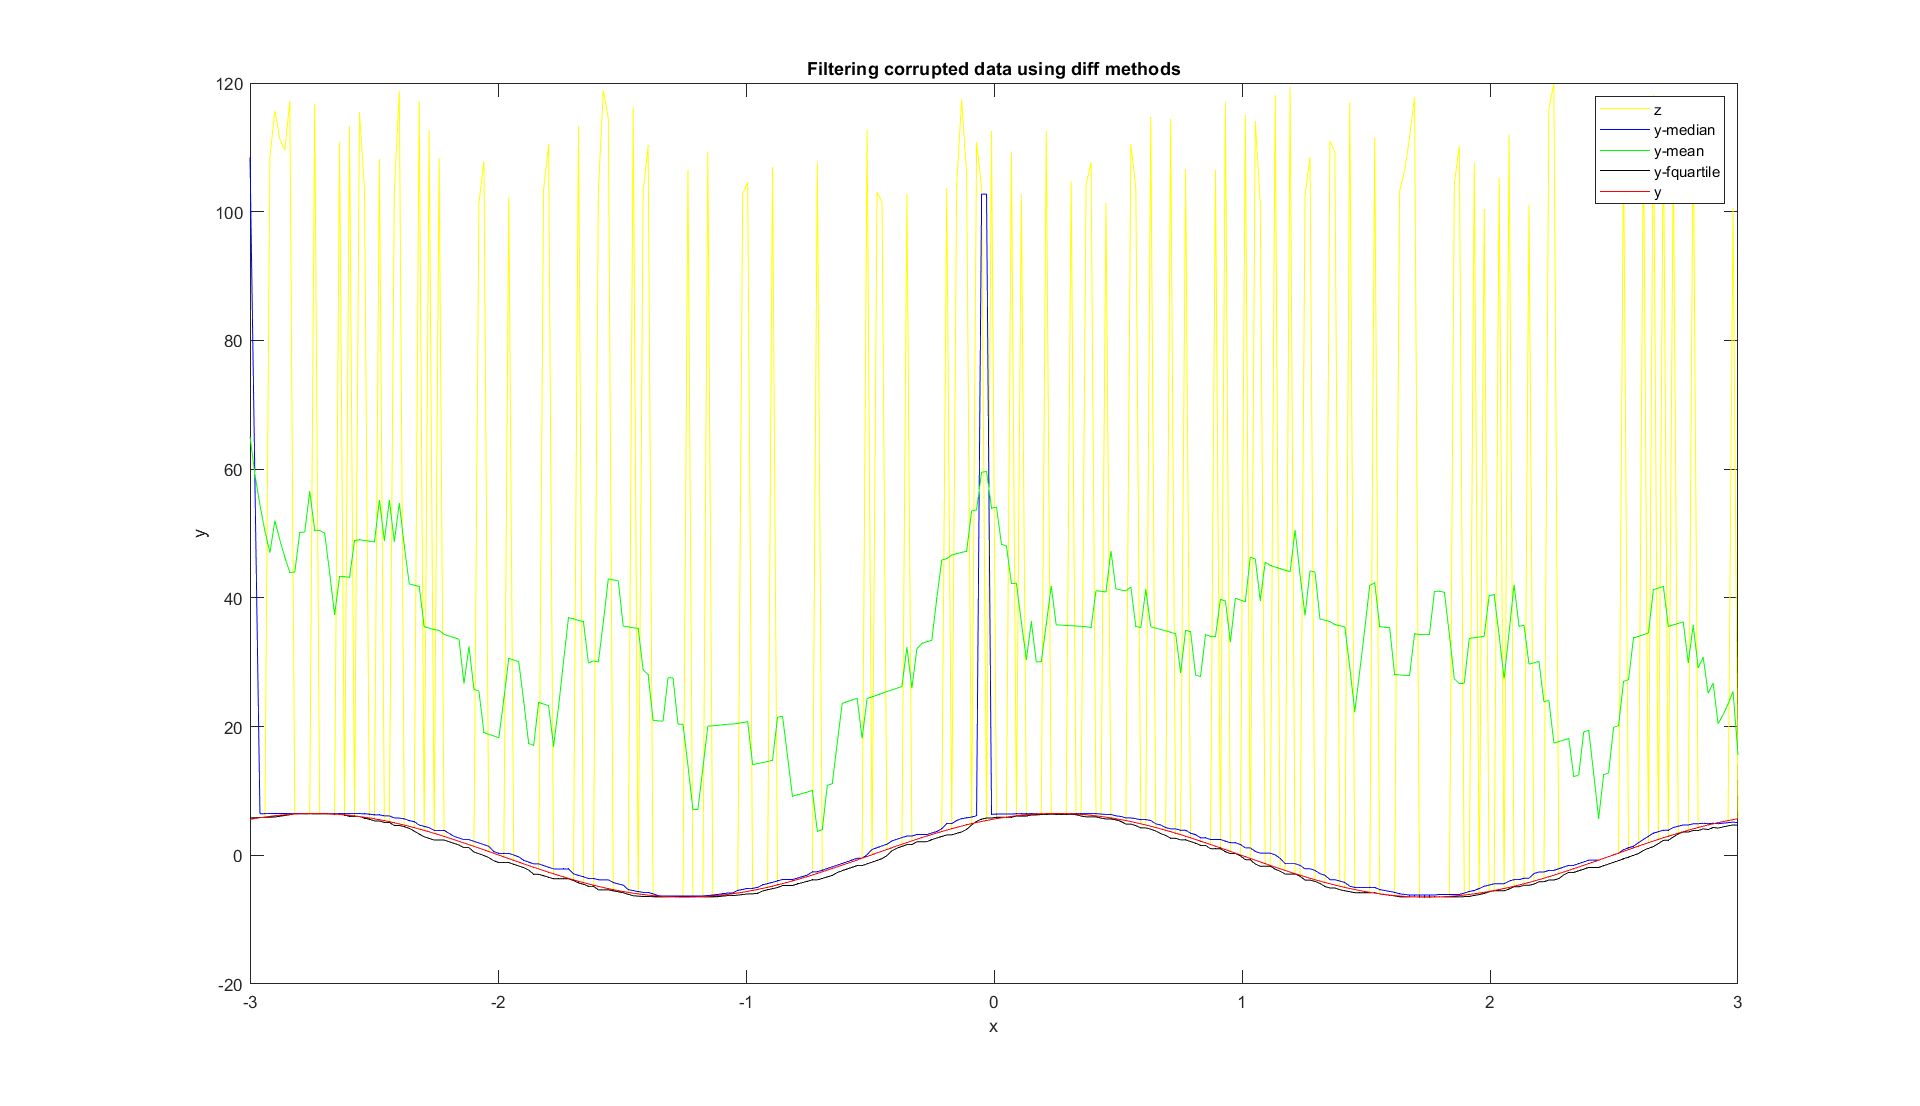
\includegraphics[width=15cm, height=8cm]{images/q6_1.png}
    \item at $f = 60\%$
    \begin{itemize}
        \item The RMS error of moving median filtering is $420.5754$.
        \item The RMS error of moving mean filtering is $215.2678$.
        \item The RMS error of moving quartile filtering is $45.1039$.
    \end{itemize}
    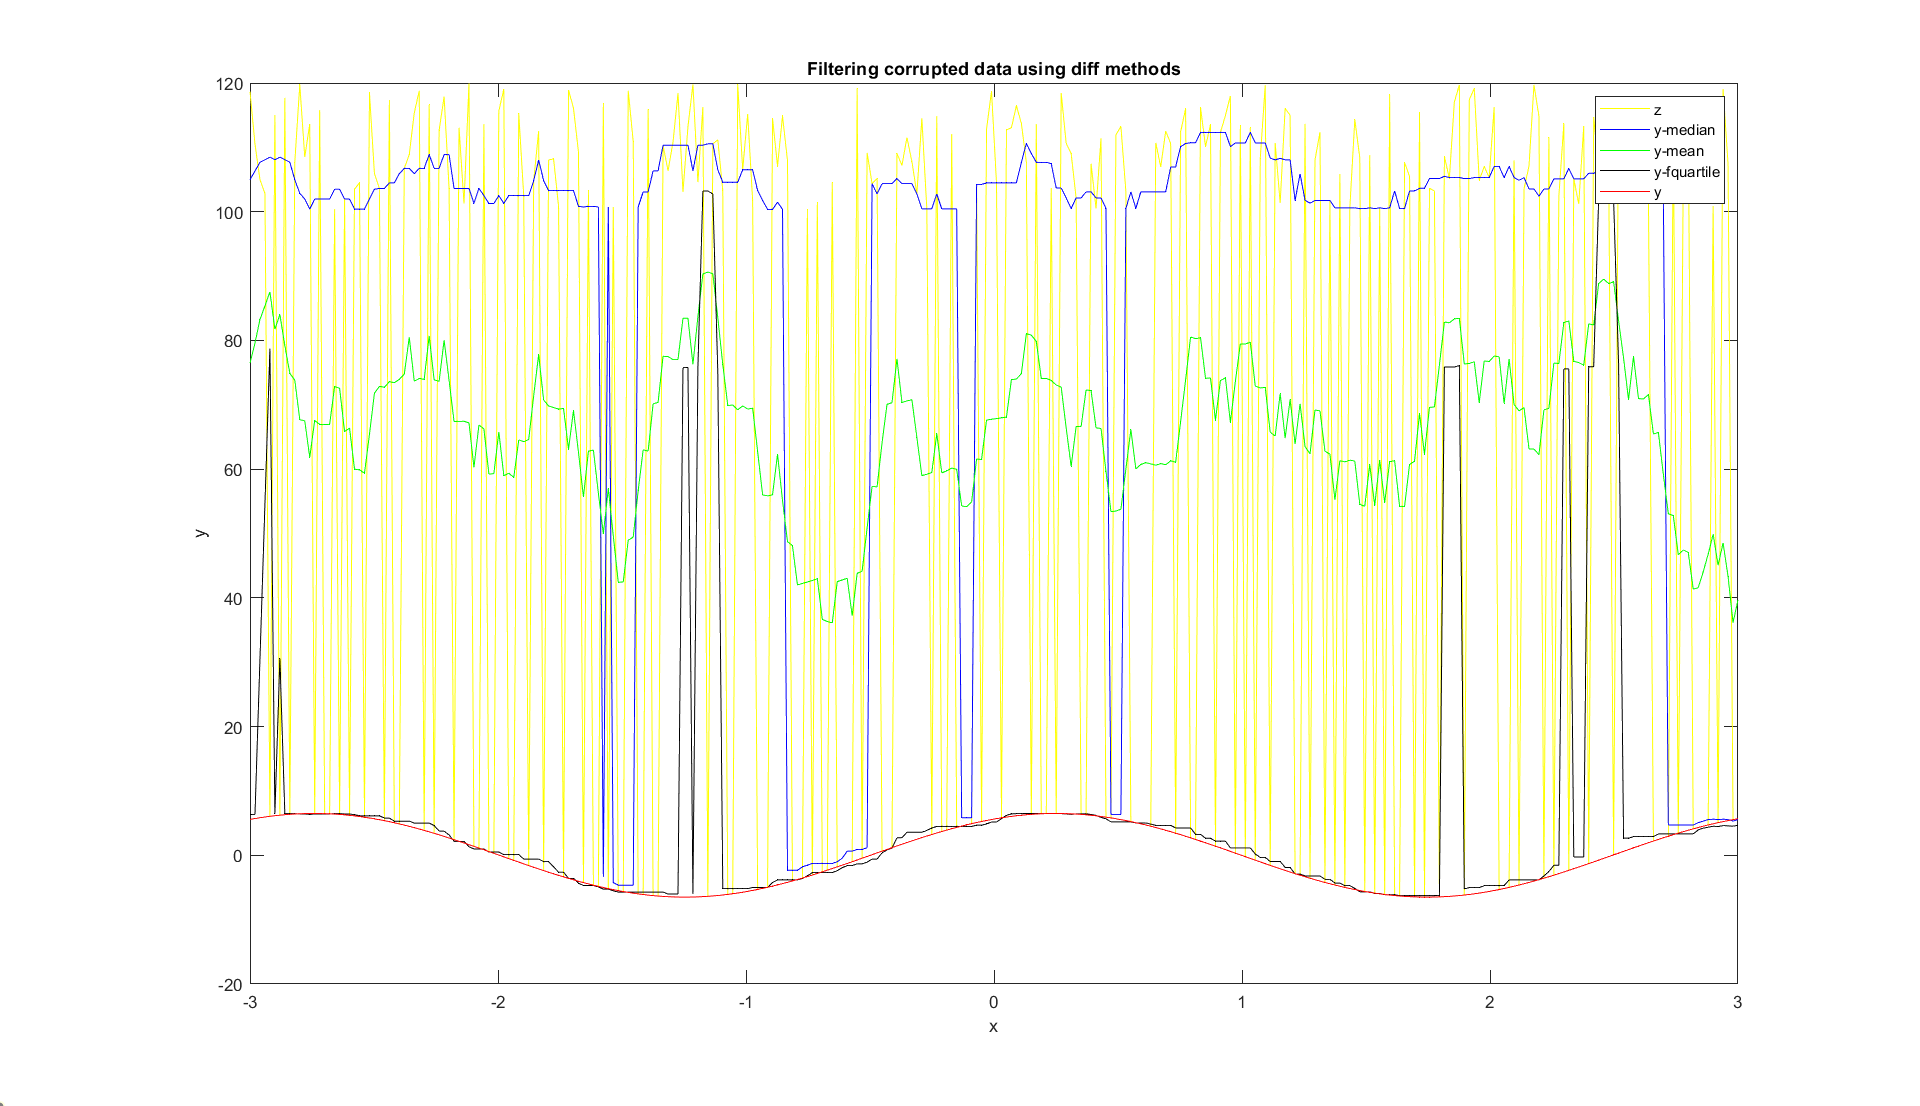
\includegraphics[width=15cm, height=9cm]{images/q6_2.png}
\end{itemize}
The moving quartile method seems to be more accurate and produces better results in RMS error. \\

The noise reduction using \emph{mean method} is least efficient since mean is more sensitive to larger noise values. The \emph{median method} in this case being more accurate since we consider the middle element by sequence, it is robust to the larger noise values. But may be inefficient in the cases of extreme noisy conditions (eg. $f = 60\%$).

And in the end, the \emph{quartile method}, which focuses on the middle 50\% of the data, is most robust against noise and outliers.

}

\end{document}